%% The following is a directive for TeXShop to indicate the main file
%%!TEX root = diss.tex

\chapter{A new taxonomy of 3D Reconstruction}
\label{ch:3DRecon_Taxo}
Existing taxonomies of 3D reconstruction techniques generally only focus on one category of techniques: ~\citeauthor{seitz2006comparison} proposed  multiple means to classify Multi-view Stereo algorithms from various perspectives. Reviews \cite{geng2011structured, salvi2004pattern} of Structured Light techniques generally classify techniques based on the type of pattern used. Photometric Stereo algorithms are classified by the assumptions or generalizations made, for instance, calibrated/uncalibrated, unknown/known reflectance, unknown/known light conditions, etc. This framework provides a means to compare intra-category algorithms, but is unsuitable to evaluate the performance of each technique across object with a range of attributes.

To have a more comprehensive understanding of the strengths and weaknesses of different techniques, a more general taxonomy is need, and one of the most popular framework categorizes 3D reconstruction techniques into active and passive methods: if the controlled light condition is used, then it's active, otherwise, it's passive. Other notable taxonomy is the spacetime framework proposed in \cite{davis2003spacetime}, which categorizes depth from triangulation techniques based on the sources of information: temporal or spatial information. Though widely adopted, the mapping of the algorithm to the conditions that works the best is generally empirical.

In the previous taxonomies, algorithms of a certain category generally work well on limited conditions, and a it's crucial to understand where algorithms perform well and where they fail. Under the previous framework, this knowledge is largely empirical, with each algorithm roughly maps to a problem domain that is poorly defined. 

The taxonomy proposed in this chapter defines the 3D reconstruction techniques based on the visual and geometric cues that techniques utilizes for reconstruction. This taxonomy transforms the 3D reconstruction problem from one requiring knowledge and expertise of specific algorithms in terms of how and when to use them, to one requiring knowledge of the visual and geometric properties of the target object.

3D reconstruction problem is classified into the following categories: stereo correspondence, shading, silhouette, texture, defocus.

\section{Stereo Correspondence}
Stereo is one of the most widely used visual cues, and is used in stereoscopy. Stereoscopy estimates the point of a 3D point by triangulation: 1). the corresponding 2D image points are detected and matched across difference views, 2). 3D line containing the center of projection and 2D projection is obtained with known camera parameters, 3). the intersection of all 3D lines is used to recover the 3D point. Trinocular and Multi-View Stereo have been introduced to improve the accuracy and robustness. However these passive approaches suffer from uniform or periodic surfaces. Active approaches overcome this problem using controlled illumination. The active techniques attempt to overcome the correspondence problem by replacing one of the cameras with a controllable illumination source, e.g., single-point laser, slit laser scanner, and temporal or spatially modulated Structured Light (SL), we refer the readers to the survey article by \citeauthor{blais2004review}. We discuss various MVS and SL techniques in the current literature.

Multi-View Stereo algorithms can be roughly categorized into four classes: volumetric based, surface evolution based, region growing based, and depthmap based methods~\cite{seitz2006comparison}.

\subsection{Multi-view Stereo}
\subsubsection{Volumetric methods}
The first class computes the cost function in a 3D volume, then extracts a surface from this volume. One successful algorithm is voxel colouring, which traverses a discretized 3D space in “depth-order” to identify voxels that have a unique colouring, constant across all possible interpretations of the scene. Another thread of work formulates the problem in the Markov Random Field (MRF) framework and extracts the optimal surface by Graph-Cut algorithms.

\citeauthor{seitz2006comparison} proposed a voxel coloring technique that traverses a discretized 3D space in “depth- order” to identify voxels that have a unique coloring, con- stant across all possible interpretations of the scene.

% - S. M. Seitz and C. R. Dyer, Photorealistic Scene Reconstruction by Voxel Coloring\\
% - Dyer's review paper on volumetric 3D reconstruction\\

\subsubsection{Surface Evolution}
The second class works by iteratively evolving a surface to minimize a cost function. The representations include voxels, level set, and surface meshes. \textit{Space Carving} technique works by iteratively remove inconsisteny voxels from the scene. \textit{Level-set} techniques cast the problem as a variational one, and use a set of PDE's as cost functions, which are deformed from an initial set of surfaces towards the objects to be detected. Other approaches represent the scene as surface meshes that moves as a function of internal and external forces. (Read Hernandez's \cite{esteban2004silhouette})

The N-view reconstruction problem is generally an ill-posed problem, which means there exists an infinite number of photo-consistent scenes. \citeauthor{kutulakos2000theory} introduced the notion of the \textit{photo hull} and the Space 
Carving algorithm that computes this least-commitment shape \cite{marr1982vision}. They can avoid to performing regularization, also ensures that the recovered 3D shape can serve as a description for the entire equivalence class of photo-consistent shapes.

Level-set based techniques minimize a set of partial differential equations defined in a volume. Like space carving methods, level-set methods typically start from a initial volume and shrink inward, or outward if the cost function is minimized. \citeauthor{faugeras2002variational} proposed a novel geometric approach based on variational principle, from which a set of PDE's can be deduced. The level set method is used to deform an initial set of surfaces towards the objects to be detected. However, level-set is no long a popular MVS technique, because high quailty models with correct topology can be directly computed from photo-consistency functions without the refinement steps.

\citeauthor{hiep2009towards} presented a visibility-based method that transforms a dense point cloud into a surface mesh, which is feed into a mesh-based variational refinement that captures small details, smartly handling photo-consistency, regularization and adaptive resolution.

% - O. Faugeras and R. Keriven, “Variational principles, surface evolution,
% pde’s, level set methods, and the stereo problem,” (level set)\\
% - C. Hernandez and F. Schmitt, “Silhouette and stereo fusion for 3d object
% modeling,”\\
% - V. H. Hiep, R. Keriven, P. Labatut, and J.-P. Pons, “Towards high-
% resolution large-scale multi-view stereo,”(graph cut)\\

\subsubsection{Region Growing}
The third class starts with a sparse set of scene points, and propagate these points to spatial neighbours and refine the cost function with respect to position and orientation. \citeauthor{furukawa2010accurate} starts from sparse, reliable seed points, and iteratively expand and filter the set of points to obtain a quasi-dense point cloud. PatchMatch Stereo and the variants start with a randomly initialized 3D volume, and make the assumption that one of the initial patch is close to the ``true'' one. This true patch can be propagated to spatial neighbours and gets refined to get closer to the optimal patch.

\citeauthor{otto1989region} proposed one of the first work on region growing stereo search. The essence of the algorithm is: start with an approximate match between a point in one image and a point in another, use an adaptive least-squares correlation algorithm to produce a more accurate match, and use this to predict approximate matches for points in the neighbourhood of the first match. Since the stereo matching algorithm is applicable for planar surfaces, it doesn't make sense to match every pixel. Therefore, they first defined a regular grid on the left image, and then defined the ``neighbourhood'' as four nearest cells in the grid.

\citeauthor{lhuillier2005quasi} presented a robust two-view quasi-dense correspondence algorithm. They first sort the list of point correspondences using the correlation score, which is called seed points. Then at each step of the propagation, they choose the best corresponding pixels from the list of seed points. Lastly, in the immediate spatial neighbourhood of the selected seed point, they look for new matches and add the bests to the list of seed points according to a combination of local constraints such as correlation, gradient disparity, and confidence. Their approach is the so-call best-first strategy, which can drastically limit the possibility of bad matches and avoid bad initialization.

PMVS is one of the first open source MVS algorithm developed by \citeauthor{furukawa2010accurate}. The goal of this method is to reconstruct at least an oriented patch at each grid cell. First, a sparse oriented patch cloud is obtained from triangulating corresponding feature points. At the expansion stage, the current patch with the best Normalized Cross Correlation score is selected and propagated to neighbouring empty cells. Lastly, two visibility-based filtering step are performed to remove erroneous patches lying outside or inside of the ``true'' surface.

PatchMatch Stereo proposed by \citeauthor{bleyer2011patchmatch} overcomes a traditional bias that pixels within a support window have the same disparity, or fronto-parallel assumption. The method is inspired by PatchMatch, which is a randomized algorithm for finding approximate nearest neighbour matches between image patches \cite{Barnes:2009:PAR}. The method starts by randomly assigning an oriented plane to each pixel in two views. Then each pixel goes through three iterations of propagations and refinement. Each pixel is propagated to the left/top or right/bottom pixels, or corresponding pixel in the second view, or a preceding or consecutive frame for stereo videos. This method can achieve sub-pixel accuracy, but is computational heavy and difficult to parallelism.

There has been some effors extending PatchMatch Stereo to multi-view scenario or proposing new propagation scheme to increase the computational efficiency. A massively parallel method using a diffusion-like propagation scheme was proposed by \citeauthor{galliani2015massively}.

% - Galliani, Massively Parallel Multiview Stereopsis by Surface Normal Diffusion\\
% - Uh, Efficient Multiview Stereo by Random-Search and Propagation\\
% - Zheng, PatchMatch Based Joint View Selection and Depthmap Estimation\\
% - Shen, Accurate Multiple View 3D Reconstruction Using Patch-Based Stereo for Large-Scale Scenes\\

\subsubsection{Depthmap Merging}
The fourth class works on the image space instead of the scene space, computes a per-view depthmap. By treating a depthmap as a 2D array of 3D points, multiple depthmaps can be considered as a merged 3D point cloud.

This method takes a set of images with camera parameters, discretizes the depth range into a finite set of depth values, then select one with maximum photo-consistency score. Uniform depth sampling may suffice for simple and compact objects. However, for complex and large scenes, a proper sampling scheme is crucial to achieve high speed and quality.

\textbf{Winner-Takes-All Depthmaps} This simple depthmap reconstruction algorithm is to evaluate photo-consistency value throughout the depth range, and pick the depth value with the highest photo-consistency score for each pixel independently. This process is call ``Winner-Takes-All'' strategy.

% \begin{figure}[h]
% \centering
% 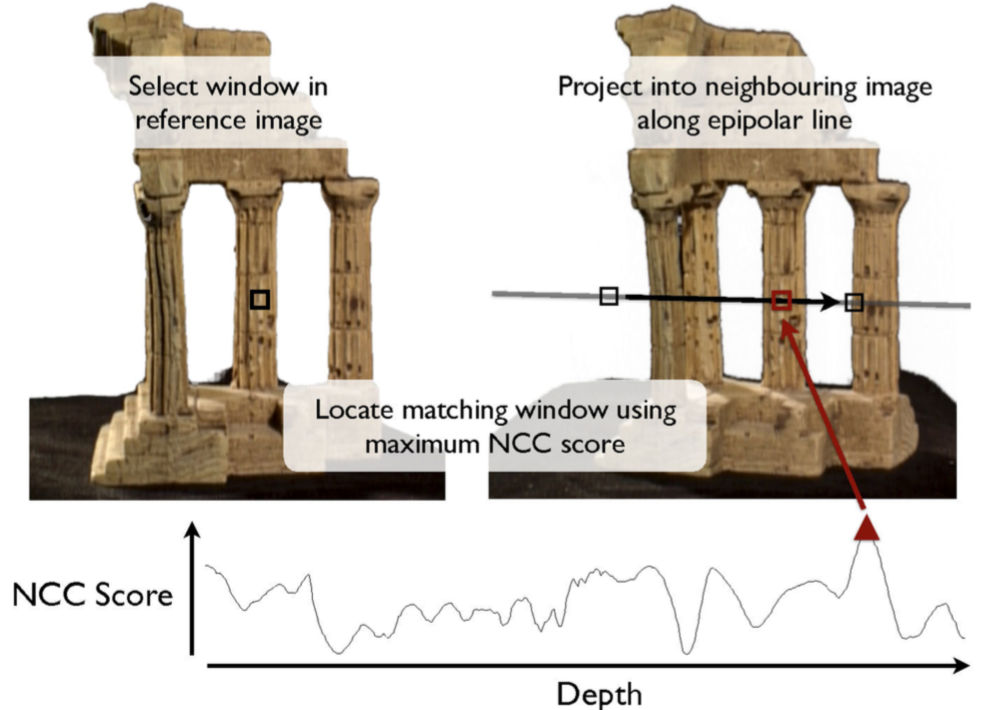
\includegraphics [width=0.7 \textwidth]{relatedwork/winner_takes_all}
% \caption{Winner-takes-all strategy for depthmap reconstruction.}
% \label{fig:winner_takes_all}\par % label should change \end{figure}
% \end{figure}

In addition to the depth value with the highest photo-consistency score, the algorithm often evaluates a confidence measure so that low-confidence depth values can be ignored or down-weighted in the merging step \cite{hu2012quantitative}. This algorithm is first proposed in by \citeauthor{esteban2004silhouette}.

Though this simplistic approach can in general achieve good enough results, it's still problematic as occlusion or non-Lambertian effects might add noise to the photo-consistency score. Therefore, a larger window size is more likely leads to a stabler match. However, the associated peak will become broader and less well localized, reducing the accuracy of the depth estimate. \citeauthor{vogiatzis2007multiview} proposed a robust photo-consistency function to overcome this problem. The basic idea is that all potential causes of mismatches like occlusion, image noise, lack of texture, or highlights are treated as outliers. Matching is treated as a problem of robust model fitting to data containing outliers. More explicitly, for each pixel in the reference image, a photo-consistency curve $S_j(d)$ is computed for each visible view $j(j\in\mathcal{N}(i))$. Since simpling avering the photo-consistency scores across various views cannot handle outliers, they build a new $\mathcal{C}$ by detecting all the local maxima $d_k$ of $S_j$, and using a Parzen window with a kernel $W$ as follows:
\begin{equation}
\mathcal{C}(d) = \sum_{j\in\mathcal{N}(i)}\sum_k S_j(d_k)W(d - d_k)
\end{equation}

This robust photo-consistency score can surpress local mixima, while simple averaging leads to erroneous results.

% \begin{figure}[h]
% \centering
% 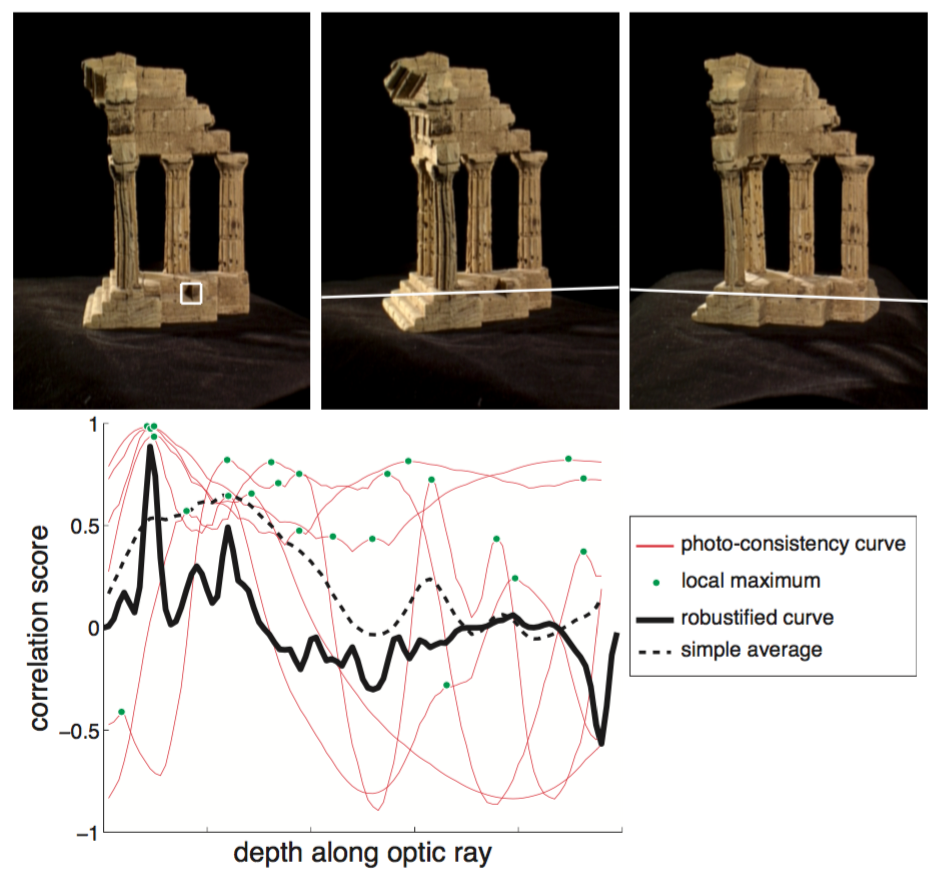
\includegraphics [width=0.7 \textwidth]{relatedwork/robust_pc}
% \caption{Robust photo-consistency function by \citeauthor{vogiatzis2007multiview}}
% \label{fig:robust_pc}\par % label should change \end{figure}
% \end{figure}

\citeauthor{goesele2006multi} proposed a simpler yet effective approach, which is to compute the average of pairwise photo-consistency scores after ignoring those below a certain threshold.

\textbf{MRF Depthmaps} In the case of severe occlusion, there may not exist a correspondence in the other images. Spatial consistency can be enforced under the assumption that neighbouring pixels have similar depth values. This can be formulated under the Markov Random Field (MRF) framework, where the problem becomes minimizing the sum of a unary $\Phi(\cdot)$ and pairwise term $\Psi(\cdot, \cdot)$. The unary term is the cost of assigning a depth label $k_p$ from a label set to the pixel $p$, whereas the pairwise term is the cost of assigning depth label $k_p$, $k_q$ to a pair of neighbouring pixels $p$ and $q$, respectively.

\begin{equation}
E(k_p)= \sum_p \Phi(k_p) + \sum_{(p,q)\in\mathcal{N}}\Psi(k_p, k_q)
\end{equation}

The unary cost reflects the photo-consistency score, which in this case, is the inversely proportional to the photo-consistency score. The pairwise term enforces the spatial regularization, thus is proportional to the amount of depth discrepancy at neighbouring pixels. 

\subsection{Structured Light}
Structured light is considered one of the most accurate reconstruction technique. It is based on projecting a temporally or spatially modulated pattern onto the surface and viewing the illuminated surface from one or more points of view. The correspondence is easily detected from the projected and imaged pattern, which is triangulated to obtain the 3D point. Each pixel in the pattern is assigned a unique codeword, and the codeword is represented (change of word) by using grey level, colour or geometric representations. Structured light is classified based on the coding strategy: time-multiplex, neighbourhood codification and direct codification \cite{salvi2004pattern}. Time-multiplexing techniques generate the codeword by projecting a sequence of patterns. Neighbourhood codification represents the codewords in a unique pattern. Direct codification techniques define a codeword for every pixel, which is equal to its grey level or colour.

\textbf{Time-multiplexing} A sequence of patterns are successively projected onto the surface, the codeword for a given pixel is formed by the sequence of illuminaiton values for that pixel across the projected patterns. This kind of pattern can achieve high accuracy due to two factors: 1). the codeword basis is small, e.g., two for binary pattern, therefore, each bit is easily distinguishable; 2). a coarse-to-fine strategy is used, and the position of the pixel becomes more precise as the patterns are successively projected. We further classify these techniques as follows: 1). binary codeword; 2). $n$-ary codeword; 3). gray code combined with phase shifting; 4). hybrid techniques.

\textbf{Spatial Neighbourhood} This kind of technique concentrate all the coding in a unique pattern. The codeword that labels a certain pixel is obtained from a neighbourhood of the pixels around it. Normally, the visual features gathered in a neighbourhood are the intensity or colour of the pixels or groups of pixels around it.

\textbf{Direct codification} There are ways that can directly represent the codeword in each pixel. To achieve this, there is a need to use either a large range of colour values or introduce periodicity. However, this kind of pattern is highly sensitive to noise because the ``distance'' between codewords is nearly zero. Moreover, the perceived colour depends not only on the projected colour, but also the intrisic clour of the surface, therefore, reference images must be taken. This kind of coding can be classified as: 1). codification based on grey levels; 2). codification based on colour.

\section{Shading Cue}
The shading variations can reveal the surface normal orientation, which can be further integrated into a 2.5D height map. Shading variation depends on the shape (surface normal orientation), reflectance (material), and lighting (illumination), therefore is generally a ill-posed problem because difference shapes illuminated under different light conditions might produce the same image. This leads to a novel technique called Photometric Stereo in which surface orientaiton is determined from two or more images. The idea of Photometric Stereo is to vary the direction of the incident illumination between successive views while holding the viewing direction constant. This provides enough information to determine surface orientation at each pixel~\cite{woodham1979photometric}. This technique can produce a surface normal map with the same resolution of the input image, \ie to produce the pixel-wise surface normal map. Since the coefficients of the normal are continous, the integrated height map can reach an accuracy that cannot be achieve by any triangulation methods. Therefore, photometric stereo is more desirable if the intrisic geometric details are of great importance.

\subsection{Photometric Stereo}
Despite the superior results achieved by Photometric Stereo,  traditional photometric stereo generally makes the following assumptions:
\begin{itemize}
\item Camera: orthographic projection, linear radiometric response
\item Reflectance: known reflectance properties, \eg Lambertian in \cite{woodham1980photometric}, specular in \cite{}.
\item Illumination: the lighting conditions are parallel rays with known directions and intensities.
\item Others: shadow, interreflection, and other global light transportation are neglected
\end{itemize}

The key problem is how to generalize the assumptions of photometric stereo. For the camera assumption, orthographic projection can be achieved by using a lens with long focus and placing the objects far from the camera. The nonlinear response can be solved by performing radiometric calibration. The shadow and other global light transportation are one of the sources of errors, some approaches consider them as outliers and remove them before normal estimation. The reflectance and lighting assumptions, however, are the most complicated ones since the reflectance properties depends on material property and the microscopic structure, and the lighting can have arbitray or fixed position, orientation, and intensity. Therefore the research on Photometric Stereo are generally on three directions: 1). traditional photometric stereo with known reflectance and lighting conditions; 2). generalization of reflectance; 3). generalization of lighting conditions.

\textbf{Traditional case} The photometric stereo is first proposed in~\cite{woodham1980photometric}. In this work, the Lambertian model is used, which is constant, and independent to incident and emit light direction.

\textbf{Generalization of Reflectance}
refer to \cite{alldrin2008photometric}

\textit{Parametric reflectance model} The reflectance is characterized by Bidirectinoal Reflectance Distribution Function (BRDF). Most BRDFs are more complicated than the Lambertian since relative few objects are either ideal diffuse or perfectly specular. The BRDF of many surfaces can be approximated as a combination of a Lambertian component and a specular component. This reflectance model has motiva{}ted a line of research~\cite{barsky20034,coleman1982obtaining,nayar1990determining}. \citeauthor{coleman1982obtaining} and \citeauthor{barsky20034} who treat specular pixels as outliers, and \citeauthor{schluns1993photometric}, \citeauthor{sato1994temporal}, and \citeauthor{mallick2005beyond} who assume the color of the specular lobe differs from the color of the diffuse lobe, allowing separation of the specular and diffuse components.

\textit{Non-parametric reflectance model} While parametric reflectance models are very good at reducing the complexity of BRDFs, they are usually only vaid for a imited class of materials. An alternative is to exploit physical properties common to a large classes of BRDFs. Typical properties include energy conservation, non-negativity, Helmholtz reciprocity, isotropy, etc. Helmholtz stereopsis, introduced by \citeauthor{zickler2002helmholtz}, is on such technique, exploiting reciprocity to obtain surface reconstruction with no dependence to the BRDF. Isotropy is another physical property which holds for material without ``grain''. \citeauthor{tan2007isotropy} use both symmetry and reciprocity present in isotropic BRDFs to resolve the generalized bas-relief ambiguity. \citeauthor{alldrin2007toward} show that isotropy, with no further assumptions on surface shape or BRDF, can be utilized to recover the surface normal at each surface point up to a plane.

\textbf{Generalization of Lighting}

The generalized lighting condition is anything other than the the ideal case of using a single distant point light source in a dark room. Therefore, any general cases like natural ambient light, multiple point light sources with/without ambient lighting, etc. To make the problem more tractable, the reflectance model should no longer be a general one, otherwise, the problem would have too many degrees of freedom, which means many different shapes with an incorrectly estimated general reflectance, and an incorrectly estimated general lighting would generate the same image appearance with much higher probability.

% [Some other papers to read] \\
% - R. J. Woodham. Photometric method for determining sur-
% face orientation from multiple images.\\
% 1. joint recovery of unknown shape and reflectance\\
% - N. Alldrin, T. Zickler, and D. Kriegman. Photometric stereo with non-parametric and spatially-varying reflectance.\\
% - D. Goldman, B. Curless, A. Hertzmann, and S. Seitz. Shape and spatially-varying BRDFs from photometric stereo.\\
% - T. Higo, Y. Matsushita, and K. Ikeuchi. Consensus photometric stereo.\\
% - B.Shi,P.Tan,Y.Matsushita,and K.Ikeuchi. Elevationangle from reflectance monotonicity: Photometric stereo for general isotropic reflectances.\\
% - BOXIN SHI's PhD thesis\\
% - Satoshi Ikehata's PhD thesis\\
% 2. a less restrained capture setup with arbitrary and unknown illumination\\
% - H. Hayakawa. Photometric stereo under a light source with arbitrary motion\\
% - T. Papadhimitri and P. Favaro. A new perspective on uncalibrated photometric stereo\\
% - B. Shi, Y. Matsushita, Y. Wei, C. Xu, and P. Tan. Self-calibrating photometric stereo\\
% 3. combine both directions\\
% - A.HertzmannandS.Seitz.Shapeandmaterialsbyexample: a photometric stereo approach.\\
% - A. Hertzmann and S. Seitz. Example-based photometric stereo: shape reconstruction with general, varying BRDFs.\\
% - W. M. Silver. Determining shape and reflectance using mul- tiple images. Master’s thesis, MIT, 1980.\\

\textbf{Shape from Shading}
The problem of recovering the shape of a surface from the intensity variation is first proposed by Horn. Most shape from shading algorithms assume that the surface under consideration is of a uniform albedo and reflectance, and that the light source directions are either known or can be calibrated by the use of a reference object. Under the assumption of distant light sources and viewer, the variation in intensity (irradiance equation) become purely a function of the local surface orientation
$$
I(x, y) = R(p(x, y), q(x, y))
$$
where $(p, q) = (z_x, z_y)$ are the depth map derivatives, and $R(p, q)$ is the reflectance map, which is often obtained from measuring or theoretical analysis.

Since there are more unknowns, additional constraints such as smoothness or integrability is required to estimate $(p, q)$.

\section{Silhouette}
\textbf{Shape from Silhouette}
In some cases, it's an easy task to perform a foreground segmentation of the object of interest, which leads to a class of techniques that reconstructs a 3D volumetric model from the intersection of the binary silhouettes projected into 3D. The resulting model is called a \textit{visual hull}.

The basic idea of shape from silhouette algorithms is that the object lies inside the intersection of all visual cones back-projected from silhouettes. Suppose there are multiple views $V$ of the target object. From each viewpoint $v\in V$, the silhouette $s_v$ can be extracted, which is the region including the object's interior pixels and delimited by the line(s) separating the object from the background. The silhouette $s_v$ are generally non-convex and can represent holes due to the geometry of the object. A cone-like volume $cone_v$ called (truncated) extended silhouette is generated by all the rays starting at the center of projection and passing through all the points of the silhouette. The target object is definitely internal to $cone_v$ and this is true fro every view $v'\in V$; it follows that the object is contained inside the volume $c_V=\cap_{v\in V}c_v$. As the size of the $V$ goes to infinity, and all possible views are included, $c_V$ converges to a shape known as the \textit{visual hull} $vh$ of the target object.

% Some approaches first approximate each silhouette with a polygonal representation and then intersect the resulting faceted conical regions in 3D space to produce polyhedral models, which can be later refined using triangular splines. Other approaches use voxel-based representations, usually encoded as octrees, because of the resulting time-space efficiency.

[computational complexity] intersection of many volumes can be slow. Simple polyhedron-polyhedron intersection algorithms are inefficient. To improve performance, most methods 1) quantize volumes, 2) perform intersection computation in 2D instead of 3D.

\subsection{Voxel based methods}
First the object space is split up into a 3D grid of voxels; each voxel is intersected with each silhouette volume; only voxels that lie inside all silhouette volumes remain part of the final shape.

\subsection{Marching intersections based methods}
The marching intersection (MI) structure consists of 3 orthogonal sets of rays, parallel to the $X$, $Y$, and $Z$ axis, which are arranged in 2D regular arrays, called the $X-rayset$, $Y-rayset$, $Z-rayset$ respectively. Each ray in each rayset is projected to the image plane to find the intersections with the silhouette. These intersections are un-projected to compute the 3D intersection between the ray and the extended silhouette on this ray. This process is repeated for each silhouette, and the un-projected intersections on the same ray are merged by the boolean AND operation.

Once the MI data structure representing the intersection of all extended silhouettes, a triangular mesh is extrated from it. This is done by the MI technique proposed in~\cite{rocchini2001marching} which traverses the ``virtual cells'' implicitly defined by the MI, builds a proper marching cube (MC) entry for them that in turn is used to index a MC's lookup table.

\begin{figure}[h]
\centering
\begin{tabular}{cc}
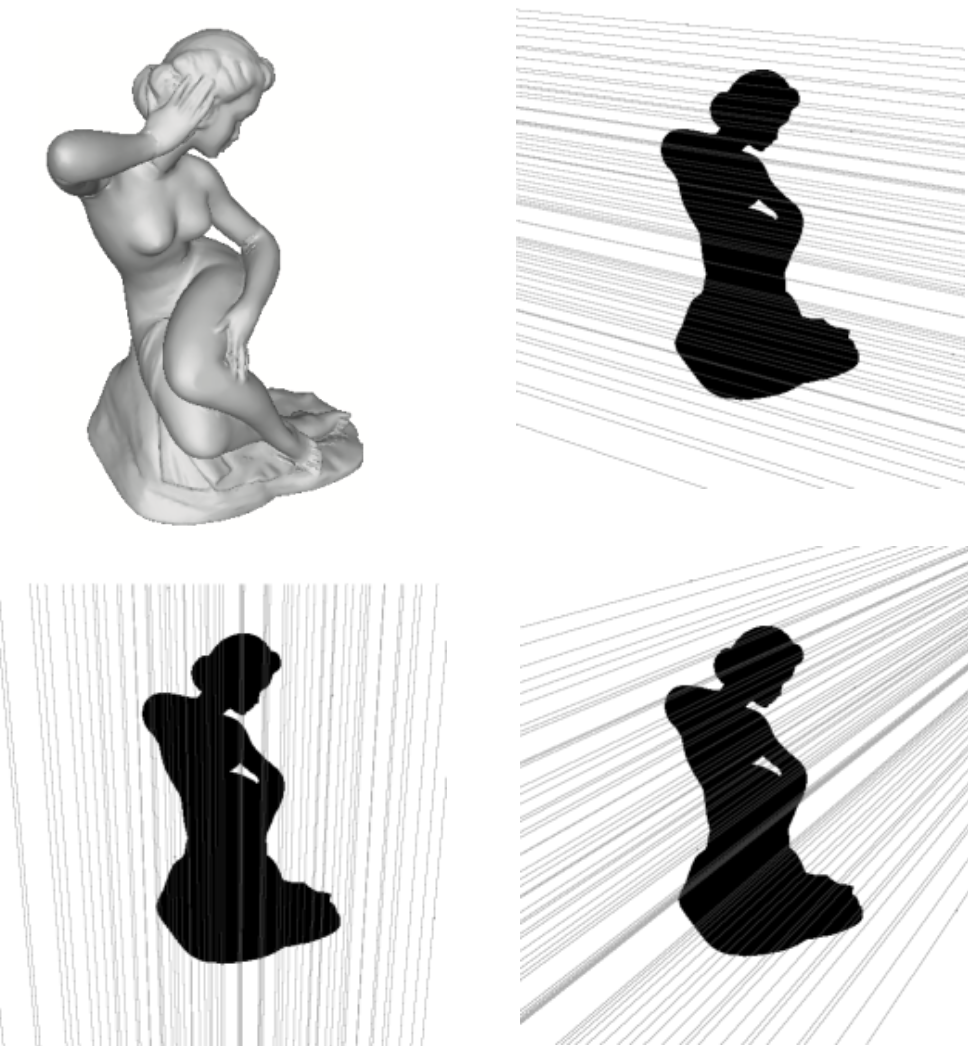
\includegraphics[width=0.5\textwidth]{taxo/scan_convert}&
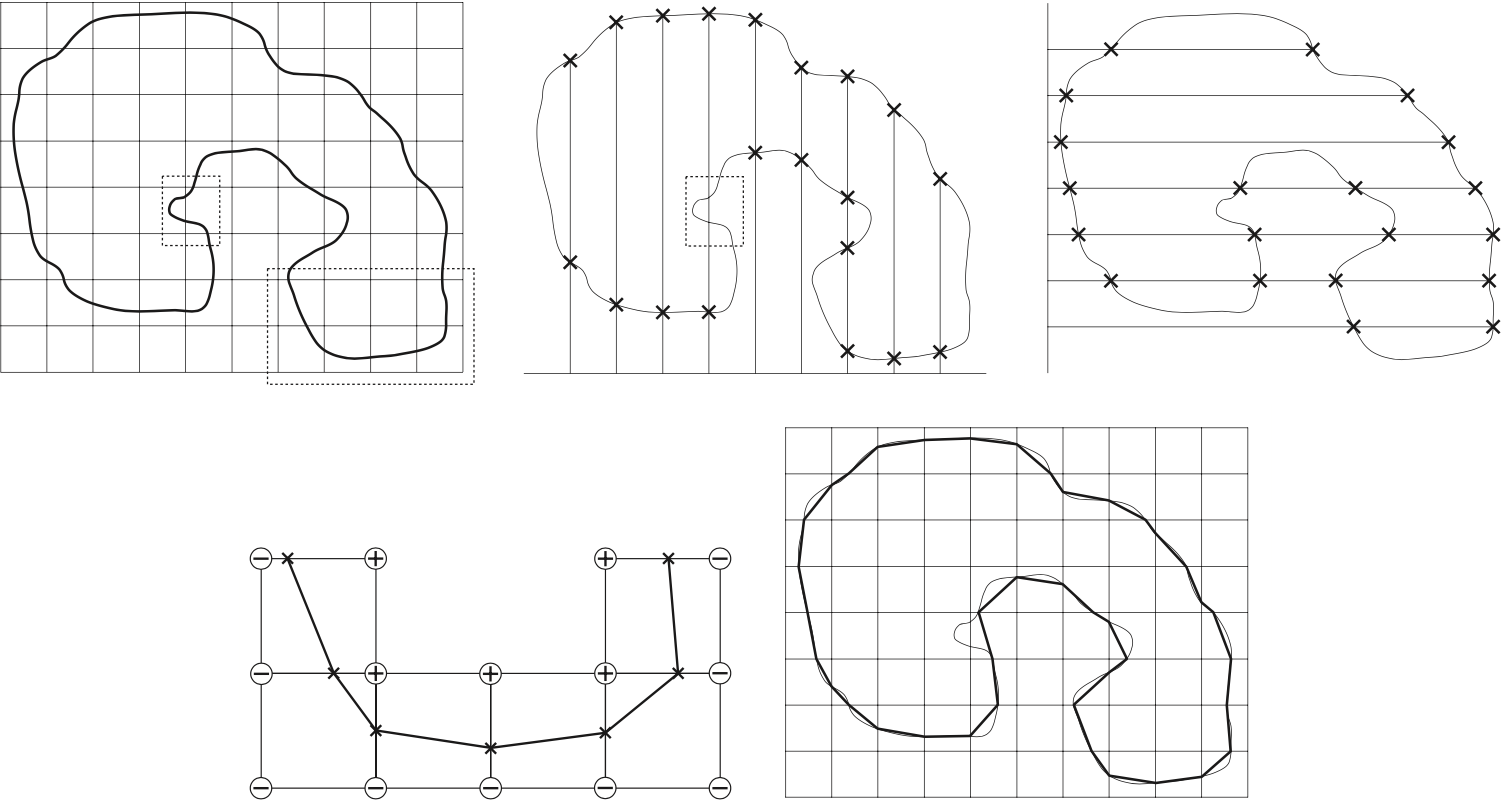
\includegraphics[width=0.5\textwidth]{taxo/mi_struct}\\
(a) & (b)\\
\end{tabular}
\caption{Illustratives of MI-based VH. (a) shows one object (top left) and its silhouette with 2D lines traced over it to find intersections along rays in the X, Y and Z ray-set of the MI, respectively. (b) shows the MI data structure and conversion algorithm in a 2D example. Image courtesy of M. Tarini.}
\label{fig:robust_pc}
\end{figure}

\subsection{Exact polyhedral methods}
The silhouette is converted into a set of convex or non-convex 2D polygons with holes allowed. The resulting visual hull with respect to those polygonal silouettes is a polyhedron. The faces of this polyhedron lie on the faces of the original cones. The faces of the original cones are defined by the center of projections and the edges in the input silhouettes. The idea of this method is: for each input silhouette $s_i$ we compute the face of the cone. Then we intersect this face with cones of all other input silhouettes, \ie a polygon-polyhedron intersection. The result of these intersections is a set of polygons that define the surface of the visual hull.

% \subsection{Image based method}
% \begin{itemize}
% \item this algorithm will only produce renderings of a visual hull from any view
% \item every pixel in the desired output image is back-projected to form a 3D ray
% \item each of those rays is intersected with each of the input silhouettes in the same way as the rays in the marching intersections method
% \item a pixel in the output image is inside the new rendering of the visual hull if its ray has any segments left in it that are intersecting the visual hull. The depth of these pixels is known from the depth of the nearest entry point on the ray.
% \end{itemize}

All of the cues above are most widely used ones, and achieved decent results. These following two cues haven't resulted in as much success. Therefore, we only discuss the general idea rather than the technical details.

\section{Texture}
\textbf{Shape from Texture}
The basic principle behind shape from texture is the \textit{distortion} of the individual texel. In general, the image formation process introduces three distortion effects: the \textit{distance effect}, which makes objects in view appear larger when they are closer to the image plane; the \textit{position effect} which makes objects appear differently when the angle between the line of sight and the image plane different; and the \textit{forshortening effect}, which distort the objects depending on the angle between the surface normal and the line of sight. Besides, different effects take place under different projection models: the orthographic projection captures only the foreshortending effect whereas the perspective projection captures all three. Therefore, shape from texture methods which use orthographic projection are valid only in a limited domain, where the other two effects can be ignored, and the perspective model captures all three effects, but the resulting algorithms are complicated and involves the solution of nonlinear equations.

\begin{figure}[h]
\centering
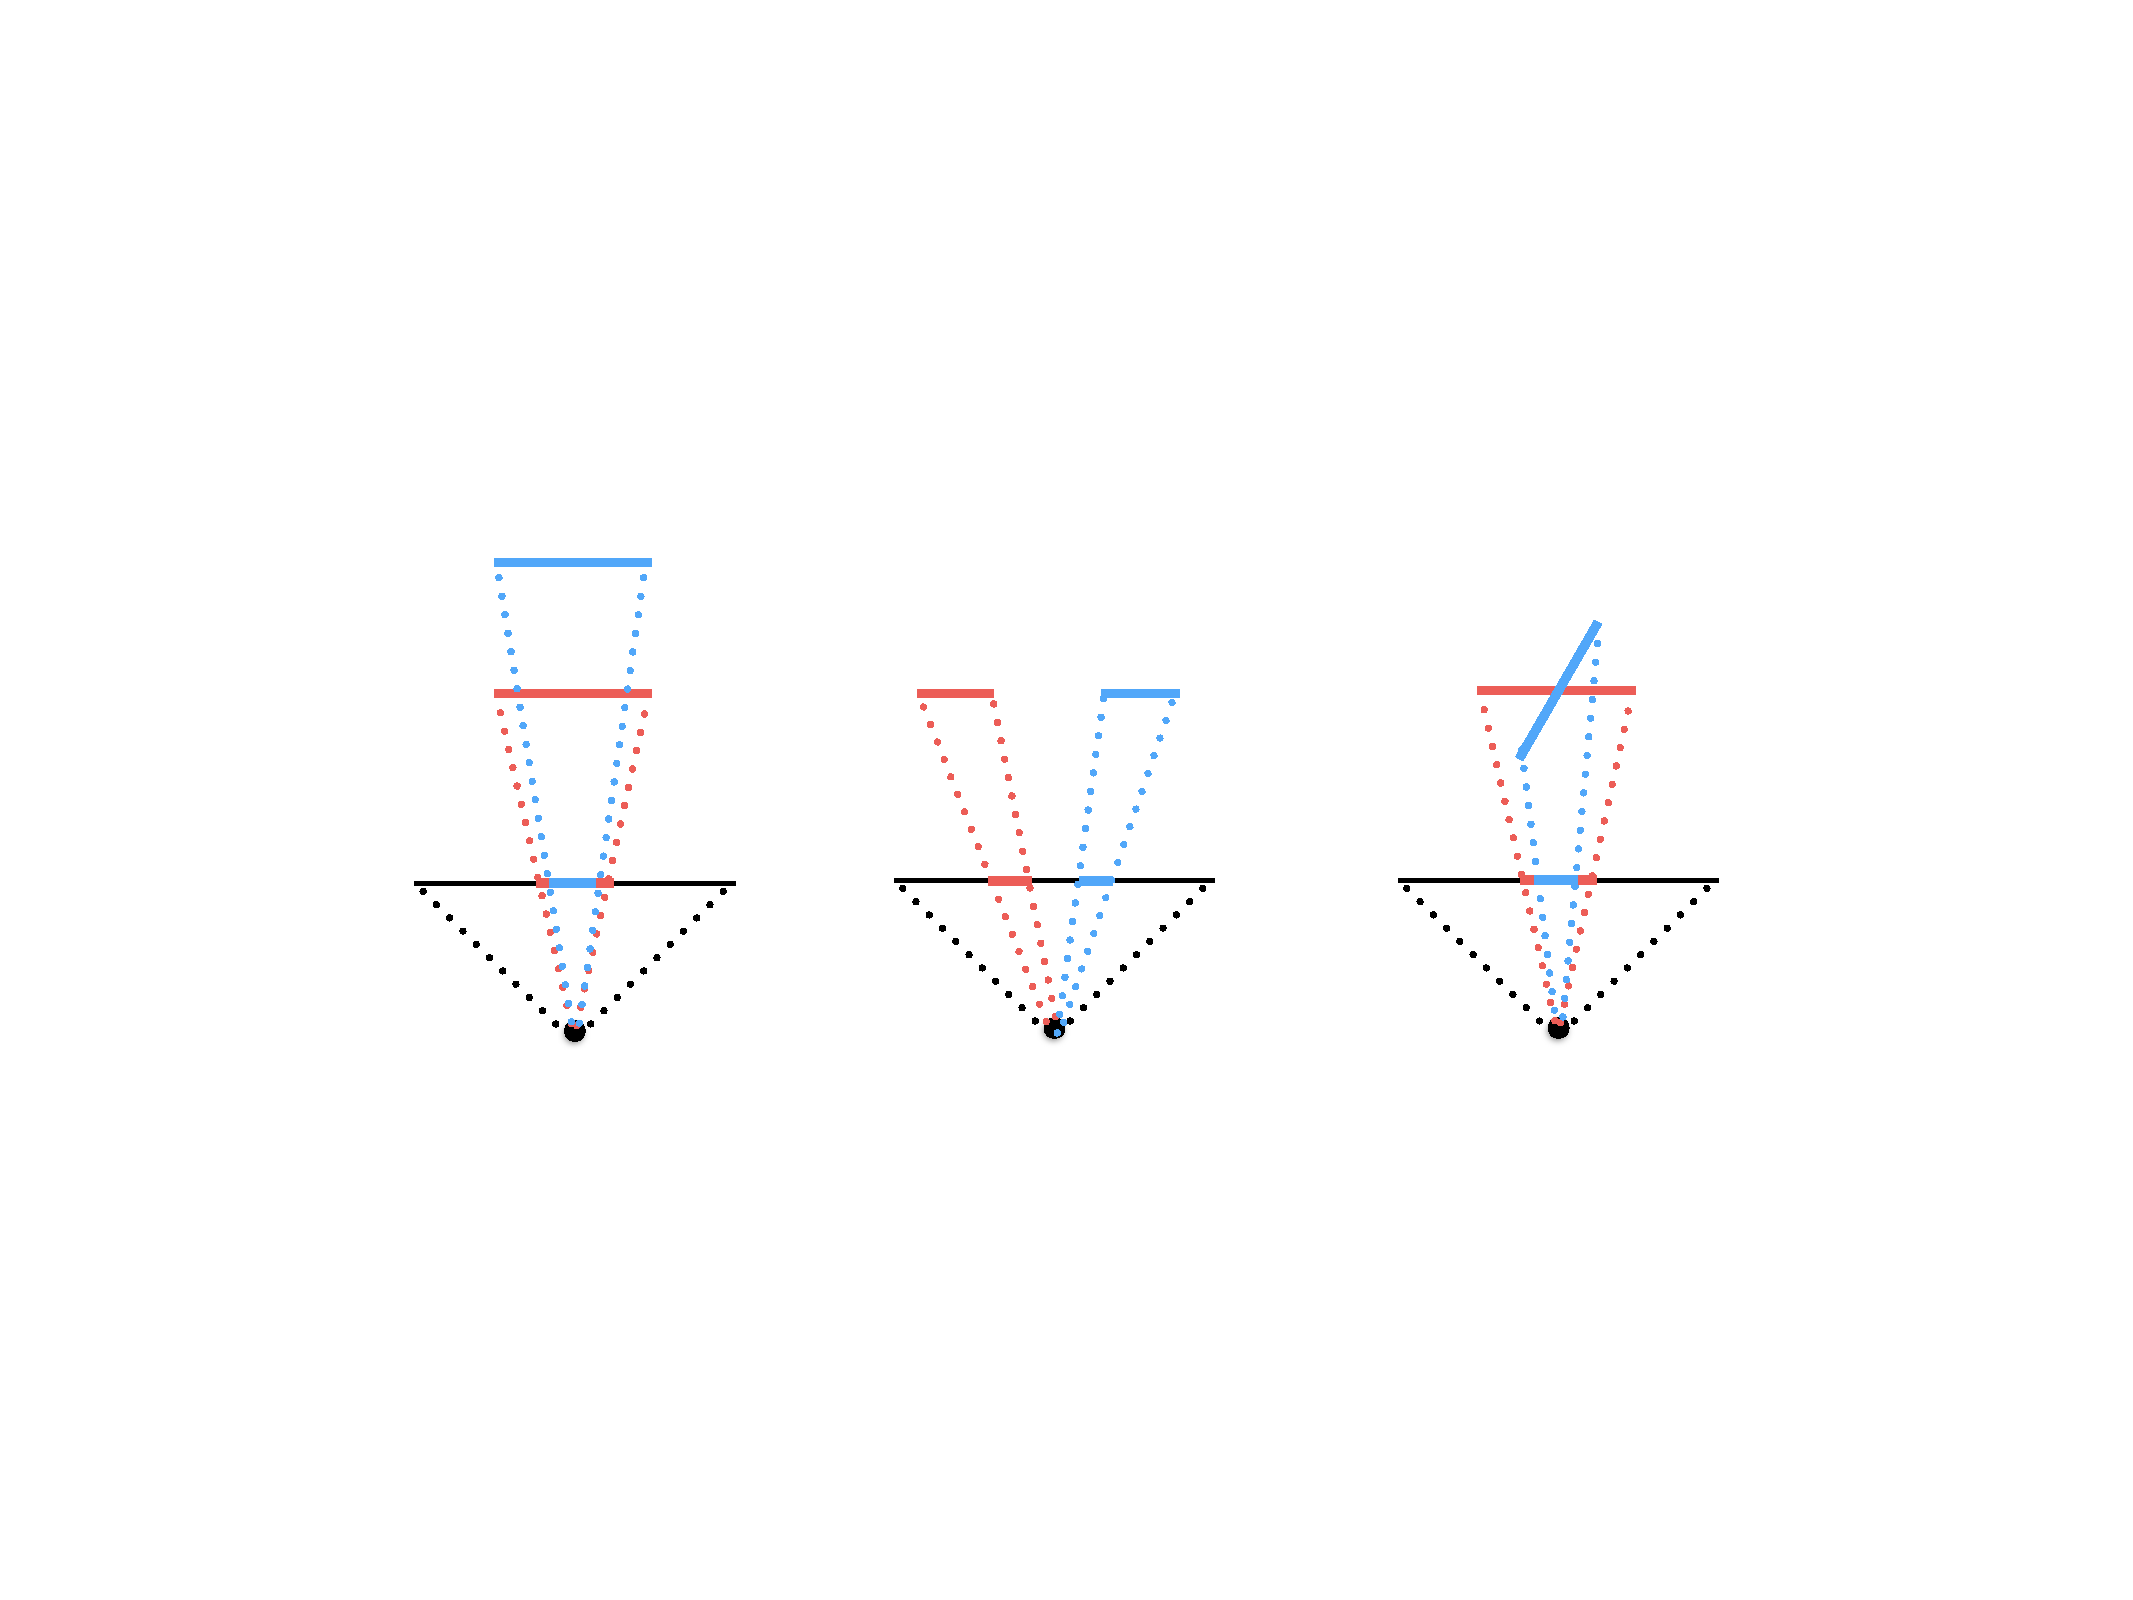
\includegraphics[width=0.8\textwidth]{taxo/tex_dist}
\caption{Three distortion effect: distance distortion, position distortion, and foreshortening distortion.}
\label{fig:tex_dist}
\end{figure}

To calculate the surface curvature at any point is far from trivial. Therefore, the surface shape is reconstructed by calculating the surface orientation (surface normal). A map of surface normals specifies the surface's orientation only at the points where the normals are computed. But, assuming that the normals are dense enough and the surface is smooth, the map can be used to reconstruct the surface shape.

\section{Defocus}
\textbf{Shape from focus}
A strong cue for object depth is the amount of blur, which increases as the object moves away from the camera's focusing distance. As shown in Figure~\ref{fig:thin_lens}, moving the object surface away from the focus plane increases the circle of confusion.

\begin{figure}[h]
\centering
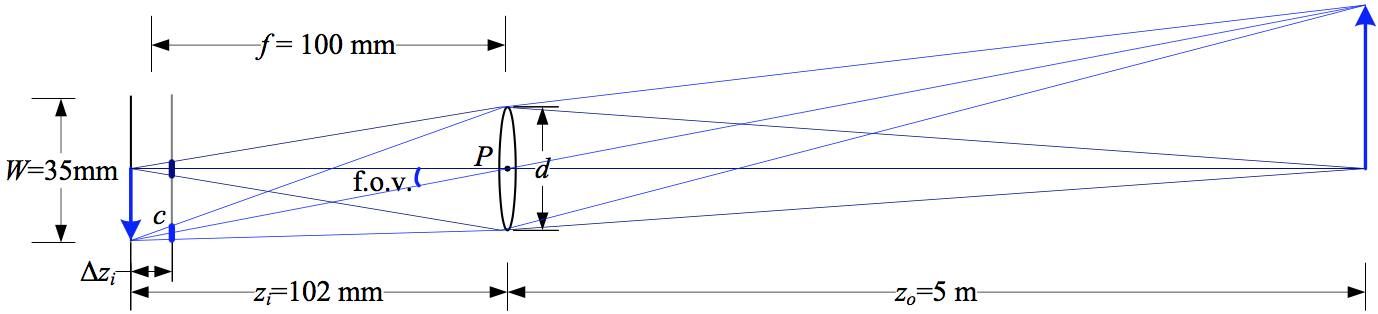
\includegraphics[width=0.8\textwidth]{taxo/thin_lens}
\caption{A thin lens of focal length $f$ focuses the light from a plane a distance $z_0$ in front of the lens at a distance $z_i$ behind the lens, where $\frac{1}{z_o}+\frac{1}{z_i}=\frac{1}{f}$. If the sensor plane moved forward $\Delta z_i$, the image are no longer in focus and the \textit{circle of confusion} $c$ depends on the distance of the sensor plane motion $\Delta z_i$ relative to the lens aperture diameter $d$.}
\label{fig:thin_lens}
\end{figure}

Figure~\ref{fig:thin_lens} shows the basic geometric image formation. The relationship between the object distance $z_o$, focal distance of the lens $f$, and the image distance $z_i$, is given by the Gaussian lens law:
$$
\frac{1}{z_o}+\frac{1}{z_i}=\frac{1}{f}
$$
All light rays that are radiated from the object and intercepted by the lens to converge at a single point on the image plane, thus a \textit{focused} image $I_f(x, y)$ is formed on the image plane. If, however, the sensor plane does not coincide with the image plane and is displaced from the image plane by a distance $\Delta z_i$, the energy received from the object is uniformly distributed over a circular patch on the sensor plane. The relationship between the radius $c$ of the circle of confusion and the sensor displacement $\Delta z_i$ is as follows:
$$
c = \frac{\Delta z_i r}{z_i}
$$
% where $r$ is the radius of the lens. If we assume that the radius $c$ of the circle of confusion is independent of the position of the object point. Therefore, the \textit{defocused} image $I_d(x, y)$ formed on the sensor plane can also be obtained by convolving the focused image $I_f(x, y)$ with a circular symmetric ``pillbox'' filter
% $$
% I_d(x, y)=p(x, y)*I_f(x, y)
% $$
% where
% $$
% p(x, y) = \begin{cases}
%     \frac{1}{\pi r^2}       & \quad \text{if } x^2+y^2\leq r^2\\
%     0  & \quad \text{otherwise}\\
%   \end{cases}
% $$
The defocused images can be obtained in three ways: by displacing the sensor with respect to the image plane, by moving the lens, or by moving the object with respect to the object plane. The first two ways cab cause the following problems:
\begin{itemize}
\item The magnification of the system varies, thereby causing the image coordinates of the object points to change.
\item The area on the sensor plane over which light energy is distributed varies, thereby causing a variation in image brightness.
\end{itemize}
To address this issue, the degree of focus is changed by moving the object with respect to a fixed configuration of the optical system and sensor. This approach ensures that the focused areas of the image are always subjected to the same magnification.

The idea is as follows: the stage is moved in increaments of $\Delta d$, and an image is captured at each stage position ($d=n\Delta d$). By studying the behaviour of the focus measure, an interpolation method is used to compute the accurate depth estimates from a small number of focus measures. An important feature of this method is the local nature, the depth estimate at an image point is computed only from focus measures recorded at that point.
\begin{figure}[h]
\centering
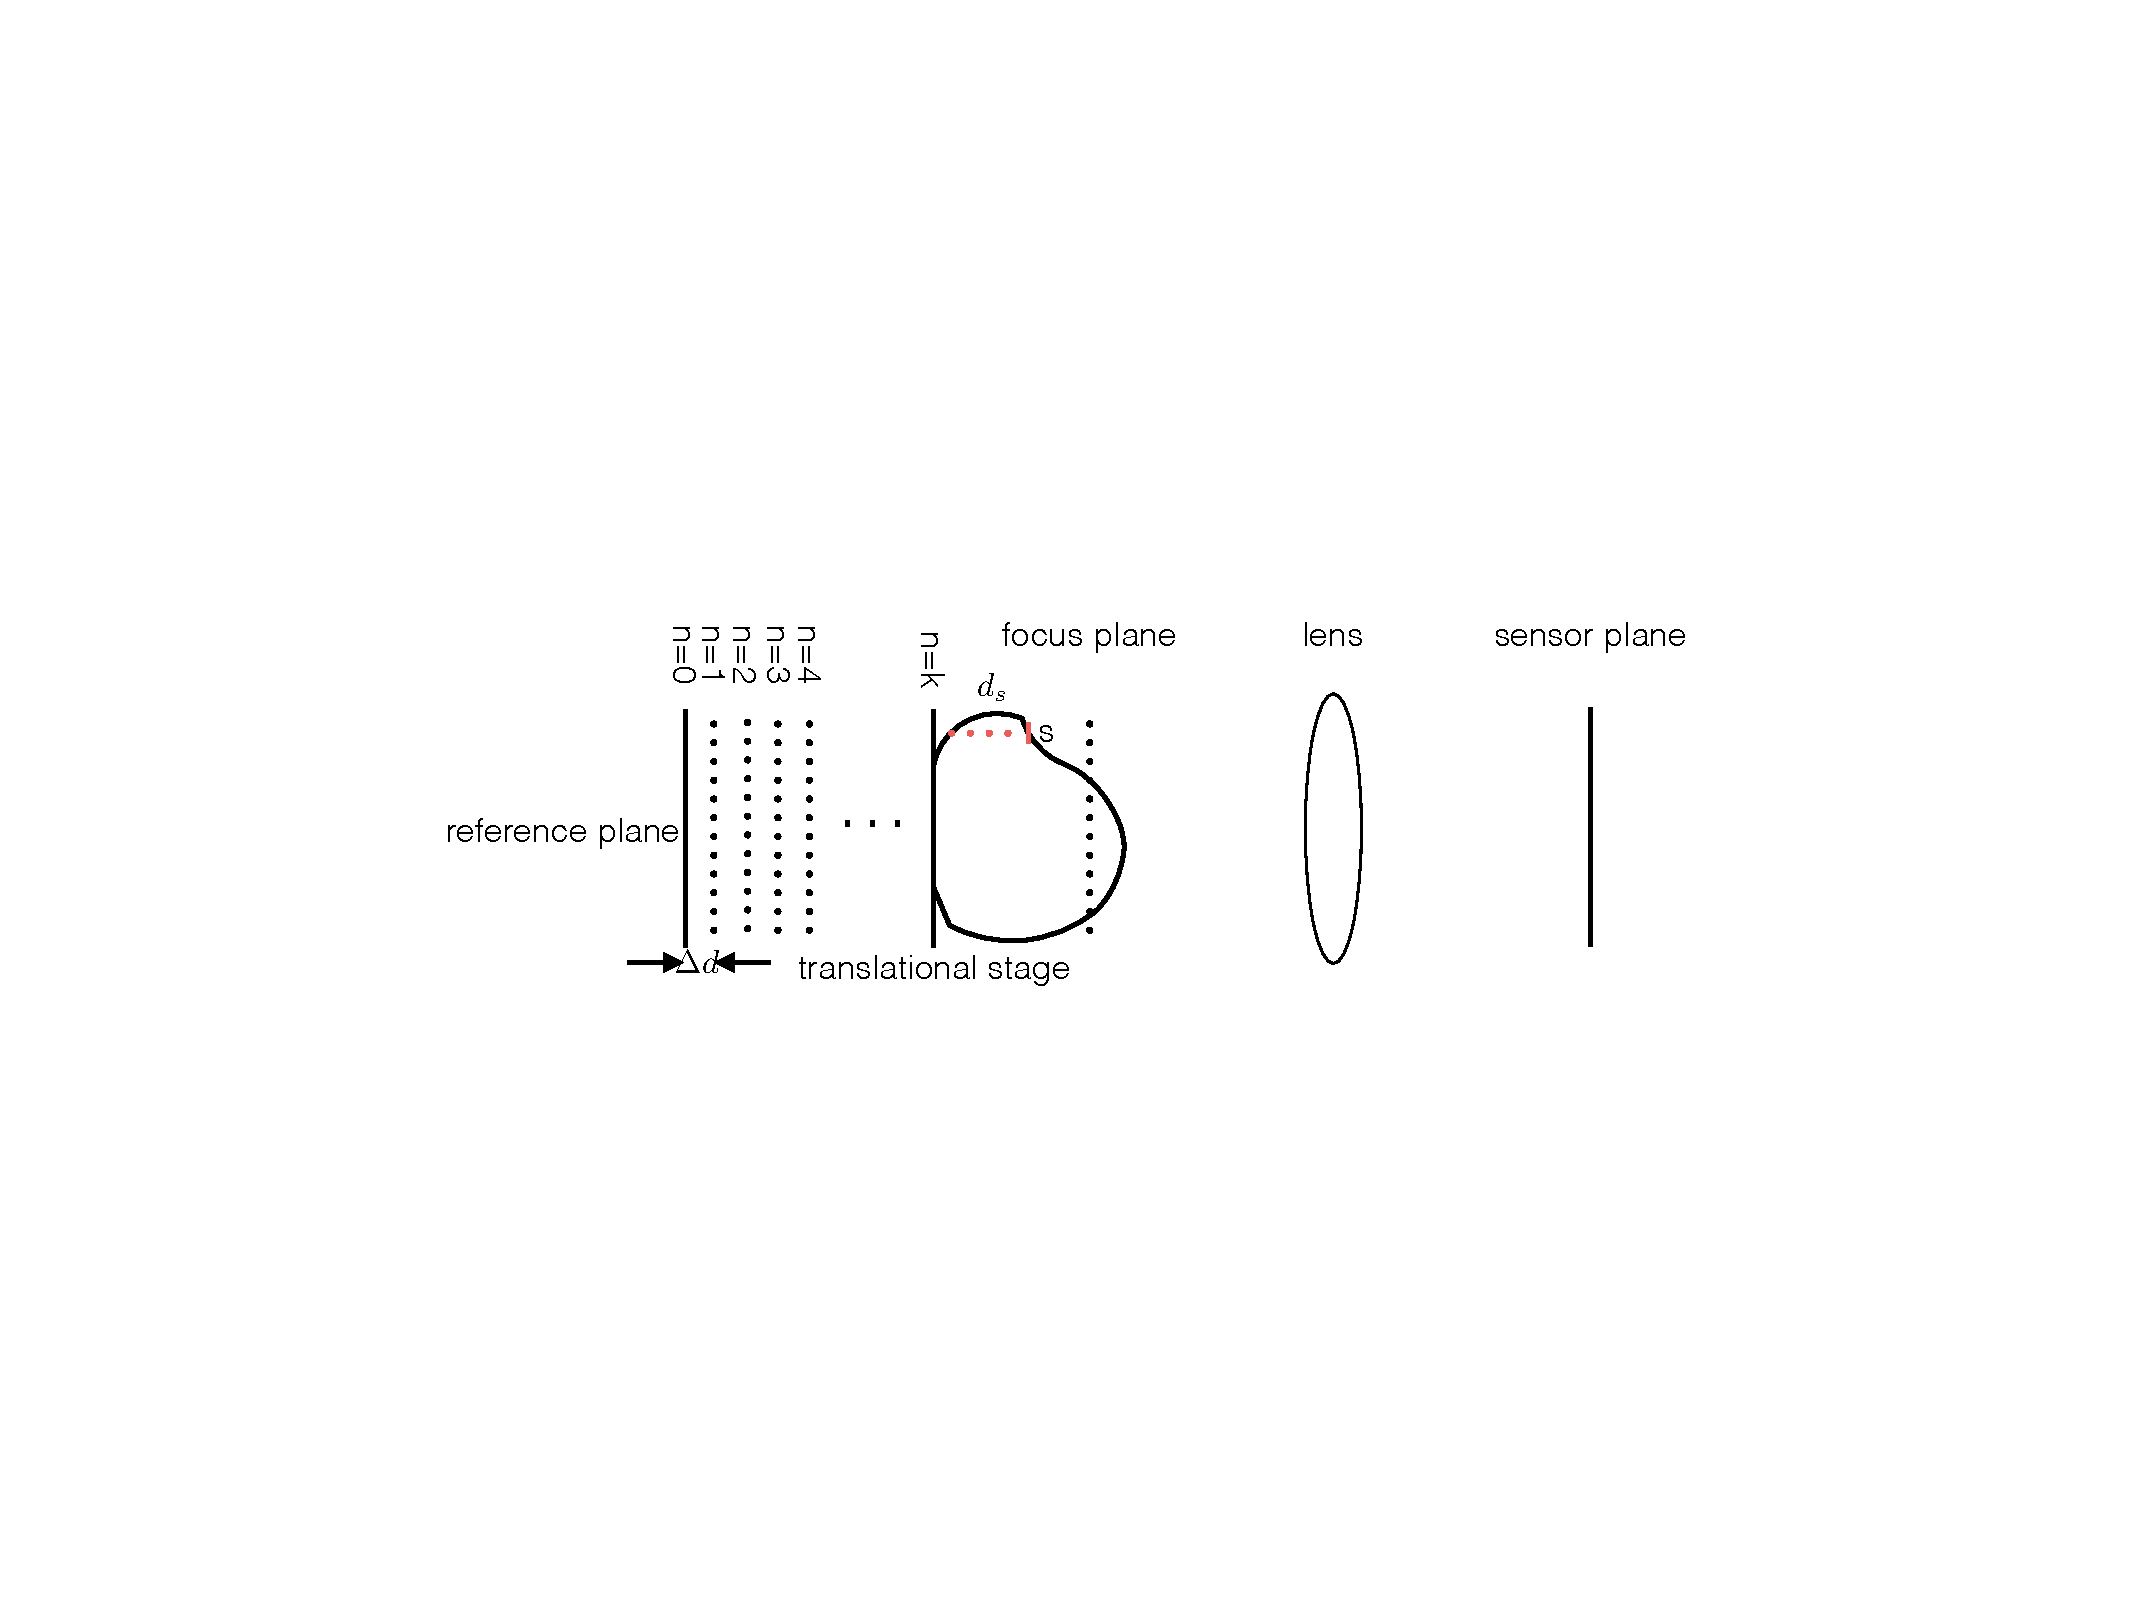
\includegraphics[width=0.8\textwidth]{taxo/shape_from_focus}
\caption{shape from focus}
\label{fig:shape_from_focus}
\end{figure}

\section{Label of Algorithms}
We propose universal labels to provide an easy way to categorize and compare 3D reconstruction techniques.

we first label the setup of the algorithm
\begin{itemize}
\item Camera: camera: $C_n$, where $n>1$ means multiple camera setup whereas $n=1$ represents single camera setup
\item Light source: light sources: $L_n$, where $n>1$ means multiple light sources whereas $n=1$ represents single light source; projector: $S$
\item Cue: stereo: ST, shading: SD, silhouette: SL, texture: T, focus: F;
\item 
\end{itemize}
\subsection{MVS}
The MVS methods can generally be classified into four classes: 1). volumetric based methods compute a cost function in a 3D volume, and extracts a surface from this volume; 2). surface evolution based methods iteratively evolve a surface/volume to minimize a cost function; 3). seed propagation based methods start with a sparse set of scene points, and perform multiple iterations of propagations and refinements; and 4) depth-map based methods compute a per-view depth map and merge multiple depth maps into a complete 3D point cloud. We use the notation below to denote each class:
\begin{itemize}
\item Reconstruction algorithm: \textbf{V}: volumetric based methods; \textbf{E}: surface evolution based methods; \textbf{P}: seed propagation based methods; \textbf{D}: depth-map based methods.
\item Surface representation: \textbf{VS}: volume scalar-field; \textbf{PC}: point cloud; \textbf{MS}: surface mesh; \textbf{DM}: depth map
\end{itemize}

For instance, voxel colouring is \textbf{V-VS}, space carving is \textbf{E-VS}, PMVS is \textbf{P-PC}.

\subsection{SL}
Structured light system overcomes the correspondence problem faced by any stereo technique by projecting a coded pattern onto the surface. The patterns are specifically designed so that codewords are assigned to a set of pixels, thus there is a direct mapping from the codewords to the coordinates of the corresponding pixel in the pattern. Based on the type of codeword used, the projection patterns are generally classified as: temporal encoding, spatial encoding, and direct encoding, refer to \cite{salvi2004pattern} for more details.

For temporal encoding, a set of patterns are successively projected onto the surface. The codeword is formed by a sequence of illumination for a specific pixel across the projected patterns. In the case of spatial encoding, the codeword of a point is obtained by considering the neighbourhood of the points around it. In the case of direct encoding, each pixel is labeled by the information representing it, which can be intensity or colour information. We use the notation below to denote each class:
\begin{itemize}
\item \textbf{Temporal encoding} (\textbf{T}): \textbf{B}: binary encoding; \textbf{N}: $n-$ary encoding; \textbf{BPS}: binary with phase shift; \textbf{H}: hybrid methods combining temporal and spatial encoding;
\item \textbf{Spatial encoding} (\textbf{S}): \textbf{NF}: non-formal codification; \textbf{DB}: methods based on  De Bruijn sequences; \textbf{M}: $M-$array;
\item \textbf{Direct encoding} (\textbf{D}): \textbf{G}: grey-level encoding; \textbf{C}: colour encoding.
\end{itemize}

The typical temporal Gray code based SL can be denoted as \textbf{T-B}.

\subsection{PS}
Almost all Photometric Stereo techniques make the following assumptions:
\begin{itemize}
\item \textbf{Camera}: orthographic projection, linear radiometric response
\item \textbf{Reflectance}: known reflectance property
\item \textbf{Illumination}: known light direction and intensity
\item \textbf{Others}: shadows, inter-reflection, and other global light transportation are neglected or considered outliers.
\end{itemize}

Thus our notation is also based on the assumptions made:
\begin{itemize}
\item Reflectance model: \textbf{L}: Lambertian model, \textbf{M}: Mixture of BRDFs
\item Illumination: \textbf{U}: uncalibrated lighting, \textbf{C}: calibrated lighting; \textbf{D}: Directional lighting, \textbf{P}: Point lighting, \textbf{E}: Environmental lighting.
\item Number of images: \textbf{S}: Small, at least three and typically 10 - 20, \textbf{M}: Medium, typically 50 - 100, and \textbf{L}: Large, typically 500 - 1000.
\end{itemize}
For example, the example-based photometric stereo can be labeled as \textbf{M-U-P-S}, the original photometric stereo is labeled as \textbf{L-C-P-S}.

\section{Summary}
Our taxonomy focuses on the visual cues detected in images, which is utilized by various techniques. Conceptualize these visual cues as dimension of the 3D reconstruction problem, we have an abstraction which allow us to think of algorithms as volumes within a $n-$dimensional problem space. Existing algorithms can be introduced into this framework based on the main visual cue used for reconstruction. Instances where these algorithms have been reported as supporting other forms of variation have been outlined, providing an initial mapping of the space that is summarized below in Table~\ref{}.

